\documentclass{standalone}
\usepackage{tikz}
\usetikzlibrary{arrows.meta, positioning, calc, shapes.multipart}

\begin{document}
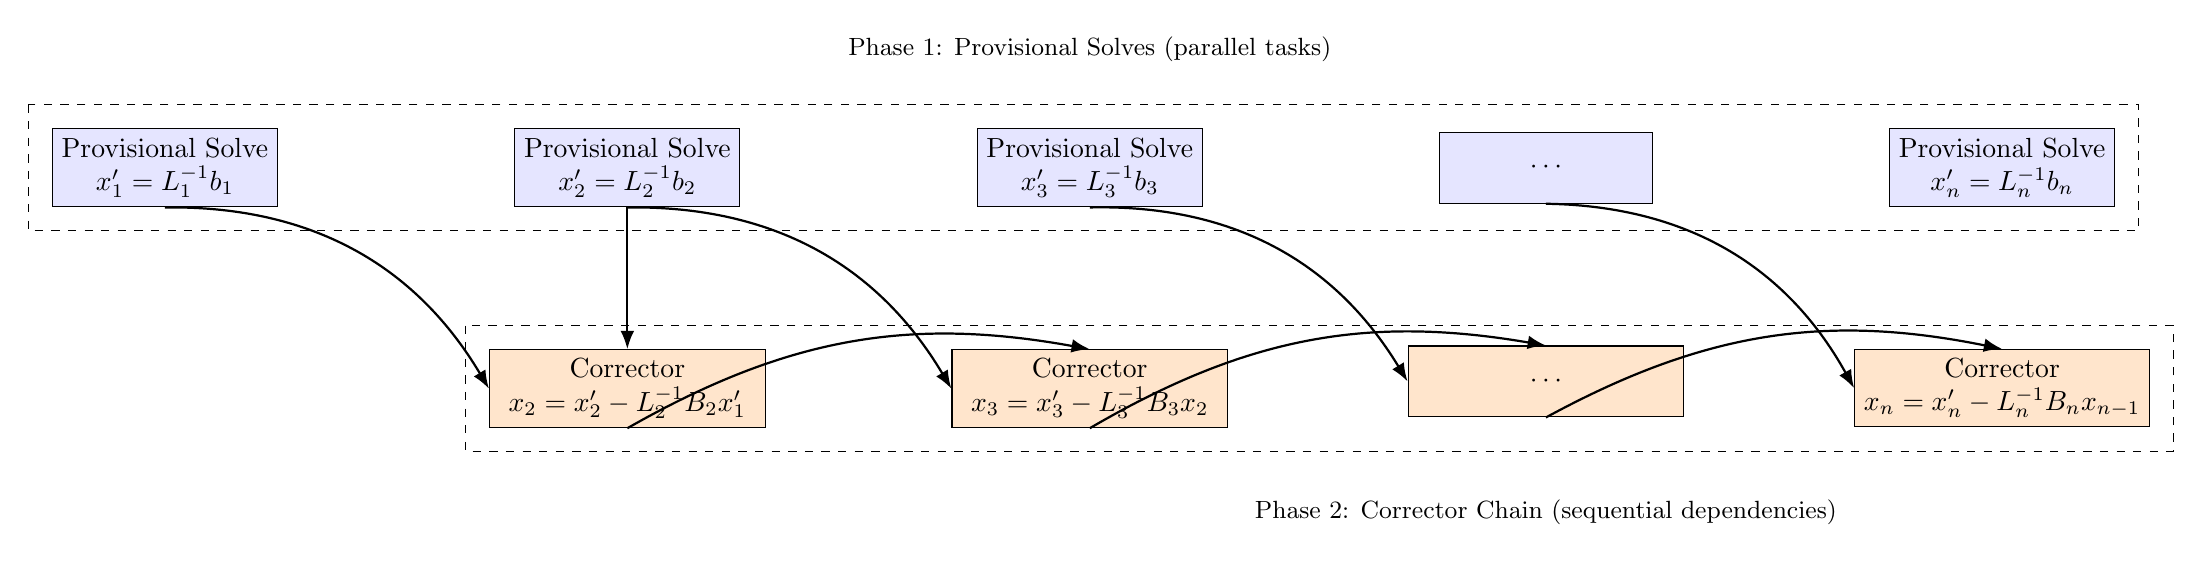
\begin{tikzpicture}[
    task/.style={rectangle, draw, fill=blue!10, minimum width=2.7cm, minimum height=0.9cm, align=center},
    corr/.style={rectangle, draw, fill=orange!20, minimum width=3.5cm, minimum height=0.9cm, align=center},
    dep/.style={-Latex, thick},
    dasheddep/.style={-Latex, thick, dashed},
    label/.style={font=\small}
]

% Provisional solves (x'_i)
\node[task] (x1) at (0,0) {Provisional Solve \\ $x'_1 = L_1^{-1}b_1$};
\node[task] (x2) [right=3.0cm of x1] {Provisional Solve \\ $x'_2 = L_2^{-1}b_2$};
\node[task] (x3) [right=3.0cm of x2] {Provisional Solve \\ $x'_3 = L_3^{-1}b_3$};
\node[task] (xdots) [right=3.0cm of x3] {$\cdots$};
\node[task] (xn) [right=3.0cm of xdots] {Provisional Solve \\ $x'_n = L_n^{-1}b_n$};

% Corrector tasks
\node[corr] (c2) [below=1.8cm of x2] {Corrector \\ $x_2 = x'_2 - L_2^{-1}B_2 x'_1$};
\node[corr] (c3) [below=1.8cm of x3] {Corrector \\ $x_3 = x'_3 - L_3^{-1}B_3 x_2$};
\node[corr] (cdots) [below=1.8cm of xdots] {$\cdots$};
\node[corr] (cn) [below=1.8cm of xn] {Corrector \\ $x_n = x'_n - L_n^{-1}B_n x_{n-1}$};

% Dependencies for x2 corrector
\draw[dep] (x1.south) to[bend left=30] (c2.west);
\draw[dep] (x2.south) -- (c2.north);

% Dependencies for x3 corrector
\draw[dep] (x2.south) to[bend left=30] (c3.west);
\draw[dep] (c2.south) to[bend left=20] (c3.north);

% Dependencies for generic cdots and cn correctors
\draw[dep] (x3.south) to[bend left=30] (cdots.west);
\draw[dep] (c3.south) to[bend left=20] (cdots.north);

\draw[dep] (xdots.south) to[bend left=30] (cn.west);
\draw[dep] (cdots.south) to[bend left=20] (cn.north);

% Labels for phase 1 and phase 2
\draw[dashed] ($(x1.north west)+(-0.3,0.3)$) rectangle ($(xn.south east)+(0.3,-0.3)$);
\node[label] at ($(x3.north)+(0,1)$) {Phase 1: Provisional Solves (parallel tasks)};

\draw[dashed] ($(c2.north west)+(-0.3,0.3)$) rectangle ($(cn.south east)+(0.3,-0.3)$);
\node[label] at ($(cdots.south)+(0,-1.2)$) {Phase 2: Corrector Chain (sequential dependencies)};

\end{tikzpicture}
\end{document}
